\documentclass[a4paper,12pt]{report}
\usepackage[a4paper,top=3cm,bottom=2cm,left=3cm,right=3cm,marginparwidth=1.75cm]{geometry}
\usepackage[brazil]{babel}
\usepackage[T1]{fontenc}
\usepackage[utf8]{inputenc}
\usepackage{amsmath}
\usepackage{amsthm}
\usepackage{amsfonts}
\usepackage{amssymb}
\usepackage{mathabx}
\usepackage{wasysym}
\usepackage{hyperref}
\usepackage{color}
\definecolor{Blue}{rgb}{0,0,0.9}
\definecolor{Red}{rgb}{0.9,0,0}
\usepackage{esvect}
\usepackage{graphicx}
\usepackage{float}
\usepackage{indentfirst}
\usepackage{caption}
\usepackage{blkarray}
\newcommand\Mark[1]{\textsuperscript#1}
\usepackage{pgfplots}
\usepackage[english, ruled, linesnumbered]{algorithm2e}
\usepackage{algorithmic}
\usepackage{multirow}
\usepackage{siunitx}
\usepackage{pdflscape}
\usepackage{booktabs}
\usepackage{makecell}
\usepackage{xltabular}
\usepackage{blindtext}
\usepackage{rccol}
\usepackage{tikz}
\usepackage{pgfplots}
\usetikzlibrary{calc}
\usepackage{galatex}
\usepackage{optidef}


\usepackage{fancyvrb}
% redefine \VerbatimInput
\RecustomVerbatimCommand{\VerbatimInput}{VerbatimInput}%
{fontsize=\footnotesize,
	%
	frame=lines,  % top and bottom rule only
	framesep=2em, % separation between frame and text
	rulecolor=\color{gray},
	%
	label=\fbox{\color{black}log.txt},
	labelposition=topline,
	%
	commandchars=\|\(\), % escape character and argument delimiters for
	% commands within the verbatim
	commentchar=*        % comment character
}

\newcommand{\nucleoe}{\emph{\text{nu }}}
\newcommand{\nucleo}{\text{nu }}
\newcommand{\imageme}{\emph{\text{nu }}}
\newcommand{\imagem}{\text{nu }}

\theoremstyle{plain}
\newtheorem{teorema}{Teorema}[section]
\newtheorem{lema}{Lema}[section]
\newtheorem{proposicao}{Proposição}[section]
\newtheorem{corolario}{Corolário}[section]

\theoremstyle{definition}
\newtheorem{definicao}{Definição}[section]
\newtheorem{observacao}{Observação}[section]
\newtheorem{exemplo}{Exemplo}[section]

\newenvironment{solucao}
{\renewcommand\qedsymbol{$\triangle$}\begin{proof}[Solução]}{\end{proof}}

\makeatletter
\renewcommand{\@chapapp}{}% Not necessary...
\newenvironment{chapquote}[2][2em]
{\setlength{\@tempdima}{#1}%
	\def\chapquote@author{#2}%
	\parshape 1 \@tempdima \dimexpr\textwidth-2\@tempdima\relax%
	\itshape}
{\par\normalfont\hfill--\ \chapquote@author\hspace*{\@tempdima}\par\bigskip}
\makeatother

\title{Introdução aos Fundamentos de Geometria de Distância}
\author{Guilherme Philippi\Mark{*}, orientado por Felipe Delfini Caetano Fidalgo\Mark{\dagger}\\Campus Blumenau\\Universidade Federal de Santa Catarina\\UFSC
	\\g.philippi@grad.ufsc.br\Mark{*}, felipe.fidalgo@ufsc.br\Mark{\dagger}}
\begin{document}
	%\iffalse
	\begin{titlepage}
		\newcommand{\HRule}{\rule{\linewidth}{0.5mm}} % Defines a new command for the horizontal lines, change thickness here
		\center % Center everything on the page
		%----------------------------------------------------------------------------------------
		%	HEADING SECTIONS
		%----------------------------------------------------------------------------------------
		\begin{flushright}
			
\includegraphics[scale=0.35]{figures/cnpq-logo.png}	
		\end{flushright}
		\vspace{-2cm}
		\begin{center}
			
\includegraphics[scale=0.22]{figures/logoufsc.jpg}
		\end{center}
		\vspace{1cm}
		
		\textsc{\LARGE \hspace{-0.17cm}Universidade Federal de Santa Catarina}\\[0.5cm] % Name of your university/college
		{\Large Centro Tecnológico, de Ciências Exatas e Educação\\ Departamento de Matemática}\\[1.5cm] % Major heading such as course name
		\textsc{\Large PIBIC \\ Relatório Final \vspace{1.5cm}  \\ }{\large Um estudo algébrico, geométrico e computacional de aplicações de Álgebras de Clifford e Geometria de Distâncias}\\[2.0cm] % Minor heading such as course title
		
		%\textsc{\LARGE Universidade Federal de Santa Catarina}\\[0.5cm] % Name of your university/college
		%{\Large Centro de Blumenau \\ Departamento de Matemática}\\[1.5cm] % Major heading such as course name
		%\textsc{\Large PIBIC \\ Programa Institucional de Bolsas de Iniciação Científica \vspace{1.5cm} \\ {\bf PROJETO DE PESQUISA}}\\[2.0cm] % Minor heading such as course title
		
		%----------------------------------------------------------------------------------------
		%	TITLE SECTION
		%----------------------------------------------------------------------------------------
		
		\HRule \\[0.4cm]
		{ \LARGE \bfseries \textbf{Uma introdução à Otimização com aplicações em Aprendizado de Máquina}} \\ [0.4cm] % Title of your document
		\HRule \\[2cm]
		
		%----------------------------------------------------------------------------------------
		%	AUTHOR SECTION
		%----------------------------------------------------------------------------------------
		
		\begin{minipage}{1\textwidth}
			\begin{center} \large
				Guilherme Philippi (guilherme.philippi@hotmail.com),
				\vspace{0.5cm}
				\\
				\underline{\textsc{Orientador:}} \vspace{0.2cm}
				Felipe Delfini Caetano Fidalgo (felipe.fidalgo@ufsc.br).
			\end{center}
		\end{minipage} \\[2cm]
		
		
		{\large \today} % Date, change the \today to a set date if you want to be precise
		
		
		\vfill % Fill the rest of the page with whitespace
		
	\end{titlepage}
	
	% \newpage
	% \pagenumbering{gobble}
	% \vspace*{\fill}
	% \begin{flushright}
	% 	\textit{Feci quod potui, faciant meliora potentes.}
	% \end{flushright}
	
	\newpage
	\pagenumbering{roman}
	
	\chapter*{Agradecimentos}
	
	Agradecimentos...
	
	Agradecimentos especiais também ao CNPq pelo incentivo financeiro da bolsa PIBIC e à 
	UFSC, por dar as condições de infraestrutura para que este projeto pudesse acontecer. 
	
	\vspace*{\fill}
	\begin{flushright}
		\textit{Feci quod potui, faciant meliora potentes.}
	\end{flushright}
	
	\newpage
	%\vspace{-1cm}
	\tableofcontents
	\newpage
	
	\begin{center}
		\large
		\textbf{Abstract}
	\end{center}
	
	\noindent This report presents a study on ..., covering everything from ... to ... We developed ... validating the applicability of the theory and consolidating the study. This work aims to contribute to ... .
	\\
	
	\noindent\textbf{Keywords:} ..., ..., ....
	
	
	\vspace{2cm}	
	\begin{center}
		\large
		\textbf{Resumo}
	\end{center}
	
	\noindent Este relatório apresenta um estudo sobre ..., abordando desde ... até ... Desenvolvemos ... validando a aplicabilidade da teoria e consolidando o estudo. Este trabalho visa contribuir para ... .
	\\
	
	\noindent\textbf{Palavras-chave:} ..., ..., ....

	\newpage
	\chapter{Introdução}\pagenumbering{arabic}
	Parágrafos:
	\begin{itemize}
		\item Introduzir Otimização matemática;
		\item Introduzir Aprendizado de Máquina;
		\item Ligar os dois temas;
		\item Apresentar a estrutura do trabalho.
	\end{itemize}
	
	\newpage
	
	\chapter{Materiais e Métodos\label{sec:materiais}}
		
	\section{Otimização}

% escrever aqui uma introdução a otimização, passando pela apresentação dos termos centrais e sobre modelagem matemática

% REVER APRESENTAÇÃO DO CLAUDIO/RAFA. BEM INTERESSANTE A ORDEM! <<<<<<

% Apresentar a introdução a modelagem modelando um problema real. Aos moldes do que Martinez fez, devemos apresentar um problema que eu tenha domínio. Bom, deve ser o problema de geometria de distâncias moleculares.. ou o problema de carteiras ótimas. Vamos ver.


A \textit{modelagem} é a área de estudo que objetiva descrever fenômenos do mundo real por meio de ferramentas matemáticas, servindo de conexão entre a matemática e as outras áreas do conhecimento \cite{meerschaert2013mathematical}. Partindo de problemas encontrados na física, engenharia, química, biologia e outras ciências, busca-se caracterizar e compreender seus comportamentos através de variáveis, funções e outras ferramentas matemáticas, abstraindo a situação real com o cuidado de que não se percam os comportamentos de interesse. Quanto mais variáveis e restrições são incorporadas para descrever os comportamentos do sistema real, mais fidedigna, porém complexa, torna-se sua representação. Grande parte da pesquisa realizada nessa área pode ser dividida em três categorias: modelos probabilísticos, modelos dinâmicos e modelos de otimização. Nos concentraremos no terceiro.

A otimização é uma área da pesquisa operacional que da suporte na tomada de decisões, com o objetivo de encontrar soluções \textit{ótimas} para um problema. Uma \textit{solução ótima} (ou \textit{ponto ótimo}) é aquela que \textit{minimiza} ou \textit{maximiza} uma função $f$, chamada de \textit{função objetivo} do problema (Figura~\ref{fig:otimizacao}). Simbolicamente, dizemos que $x^* \in \mathcal{X}$ é um \textit{ótimo global} do problema de minimizar $f$, restrito a $\mathcal{X}$, se satisfaz 
\begin{equation}
	f(x^*)\leq f(x)\text{ para todo } x\in \mathcal{X}.
\end{equation} O conjunto $\mathcal{X}$ é chamado de \textit{espaço de busca} por uma solução, e encontrar essa solução ótima nem sempre é fácil ou mesmo possível. Isso gera a necessidade do estudo de \textit{aproximações} para as soluções ótimas de um problema \cite{elizabeth2013otimizaccao}.  

Perceba que o problema de maximizar $f$ é equivalente ao de minimizar $-f$ (veja Figura~\ref{fig:max_min_equiv}), o que nos permite abster de comentários sobre um dos dois nas definições e proposições que seguem. Por lealdade à abordagem dos colegas da Unicamp, focaremos exclusivamente na apresentação orientada pela minimização, deixando os equivalentes de maximização como exercício para o leitor. 

\begin{figure}[h]
	\centering
	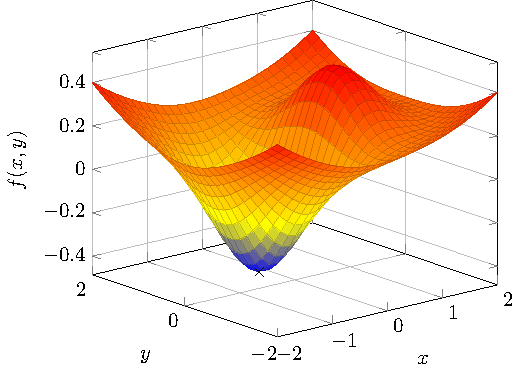
\includegraphics[scale=0.9]{secOtimizacao/figures/solucaoOtima.pdf}
	\caption{Ilustração do problema de minimização para a função objetivo $f:\mathbb{R}^2\to\mathbb{R}$, definida pelo mapeamento $(x,y) \mapsto xe^{-x^2-y^2} + \frac{x^2 + y^2}{20}$.}
	\label{fig:otimizacao}
\end{figure}

\begin{figure}[h]
    \centering
    \begin{tikzpicture}[scale=1.5]
        % Eixo x
        \draw[->] (-1,0) -- (3,0) node[right] {$x$};
        % Eixo y
        \draw[->] (0,-1) -- (0,1) node[above] {$f(x)$};
        % Função f(x)
        \draw[domain=-0.5:2.5,smooth,variable=\x,blue] plot ({\x},{0.4*(\x-1)^2 - 0.5}) node[right] {$f(x)$};
        % Função -f(x)
        \draw[domain=-0.5:2.5,smooth,variable=\x,red] plot ({\x},{-0.4*(\x-1)^2 + 0.5}) node[right] {$-f(x)$};
        % Ponto máximo
        \filldraw[black] (1,0.5) circle (1pt) node[above right] {Máximo};
        % Ponto mínimo equivalente
        \filldraw[black] (1,-0.5) circle (1pt) node[below right] {Mínimo equivalente};
    \end{tikzpicture}
    \caption{Maximizar $f(x)$ é equivalente a minimizar $-f(x)$.}
    \label{fig:max_min_equiv}
\end{figure}
	
Assim, um problema geral de otimização é representado como 
\begin{mini}
	{x\in \mathcal{X}}{f(x)}{}{}
\end{mini}
onde $x$ é o vetor de variáveis contidas no \textit{espaço de busca} $\mathcal{X} \subset \mathbb{R}^n$, candidatas a solução. Dependendo da natureza do problema, podemos representar o conjunto $\mathcal{X}$ através de restrições de igualdade e de desigualdade, ou seja,
$$\mathcal{X} = \{x\in \mathbb{R}^n\ |\ c_\mathcal{E}(x) = 0,\ c_\mathcal{I}(x) \leq 0\},$$
onde $c_\mathcal{E}: \mathbb{R}^n\to\mathbb{R}^m$ e $c_\mathcal{I}: \mathbb{R}^n\to\mathbb{R}^p$ são as \textit{funções de restrição} do espaço de busca $\mathcal{X}$ e $0$ representa os vetores nulos de dimensão apropriada\footnote{A menos de ambiguidades, omitiremos as dimensões de vetores nulos e de identidades.}.
Para destacar as restrições do problema, iremos escrevê-lo como 
\begin{mini}
	{x\in \mathbb{R}^n}{f(x)}{}{}
	\addConstraint{c_\mathcal{E}(x) = 0}
	\addConstraint{c_\mathcal{I}(x) \leq 0.}
\end{mini}

O subconjunto de $\mathbb{R}^n$ que satisfaz todas as funções de restrição também é chamado de \textit{conjunto factível} (ou viável) do problema. No entanto, caso $\mathcal{X} = \mathbb{R}^n$, dizemos que esse é um \textit{problema de otimização irrestrito}. A otimização irrestrita é de suma importância para a área, visto que uma das técnicas existentes para solucionar problemas com restrição é reescreve-los como problemas irrestritos associados \cite{elizabeth2013otimizaccao}.
Além disso, também podemos intercambiar restrições de igualdade e desigualdade livremente, já que restrições de igualdade podem ser reescritas como duas de desigualdade
$$h(x)=0 \quad \iff \quad \begin{matrix}
	\ h(x) \leq 0\\
	-h(x)\leq 0,
\end{matrix}$$
e restrições de desigualdade podem ser reescritas como uma igualdade, mediante a introdução de variáveis artificiais ``de folga''
$$g(x) \leq 0 \quad \iff \quad g(x) + z^2 = 0,\ z\in \mathbb{R}. $$
Infelizmente, substituições como essas costumam ser indesejadas tanto do ponto de vista teórico como do ponto de vista computacional \cite{izmailov2005otimizaccao}.
\\

Vejamos um clássico exemplo de otimização, cuja aplicação econômica denuncia a importância e alcance da área. 

\begin{exemplo}[Lucro de produção]\label{ex:custoproducao}
	Considere que uma fábrica produza $p_1,p_2$ produtos distintos, cujos respectivos lucros por unidade sejam de $l_1 = 10,l_2 = 15$, e que cada produto $p_1$ requer 2 horas de trabalho manual e 1 hora nas máquinas para ser produzido, enquanto cada $p_2$ requer 3 horas de trabalho e 2 horas na máquina. Sejam $t_1 = 100, t_2 = 60$ as respectivas horas disponíveis de trabalho manual e de máquina. Formule um problema de otimização que decida as quantidades $p_1,p_2$ a fim de maximizar o lucro da fábrica.

	\begin{solucao}
		A função objetivo $l$ que queremos maximizar é o lucro total. Ou seja, é a função
		\begin{align*}
			l: \mathbb{R}^2 &\to  \mathbb{R}\\
			(p_1,p_2) &\mapsto l_1p_1 + l_2p_2 = 10p_1 + 15p_2.
		\end{align*}
		Como $p_1,p_2$ são quantidades de produtos produzidos, devem ser não negativos: $$p_1\geq0 \quad \text{e}\quad p_2 \geq 0.$$ Além disso, temos duas restrições relativas às horas disponíveis $t_1,t_2$, descritas por $$2p_1 + 3p_2 \leq t_1 = 100 \quad 1p_1 + 2p_2 \leq t_2 = 60.$$ 

		Dessa forma, nosso problema de otimização pode ser descrito como
		\begin{maxi}
			{(p_1,p_2)\in \mathbb{R}^2}{10p_1 + 15p_2}{}{}
			\addConstraint{2p_1 + 3p_2 \leq 100}
			\addConstraint{1p_1 + 2p_2 \leq 60}
			\addConstraint{p_1\geq 0}
			\addConstraint{p_2\geq 0.}
		\end{maxi}
	\end{solucao}
\end{exemplo}

As restrições $p_1,p_2\geq 0$ do exemplo acima são comuns a vários problemas, e chamamos elas de restrições de não negatividade das variáveis. Também, nesse exemplo, o conjunto factível resultante é um subconjunto de $\mathbb{R}^2$, cuja continuidade induz uma busca contínua por valores ótimos nesse conjunto. Problemas desse tipo são chamados de \textit{problemas de otimização contínua}. Em contraste, quando nosso espaço de busca é um subconjunto dos inteiros $\mathbb{Z}$, ou, mais geralmente, quando o conjunto de restrições é tal que nosso espaço factível é um conjunto enumerável de pontos, diremos que esse é um \textit{problema de otimização discreta}.

\begin{exemplo}[Problema da Mochila (\textit{Knapsack problem})]
	Sejam $x_1,\dots,x_n$ items com pesos $w_1,\dots,w_n$ e valores $v_1,\dots,v_n$. Se uma mochila suporta um peso máximo $w_\text{max}$, modele o problema de escolher quais items devem ser colocados na mochila de forma a maximizar o valor total dos itens, respeitando a restrição de peso.
	\begin{solucao}
		Para representar as $n$ escolhas de itens que estarão na mochila, usaremos uma sequência $x_1,\dots,x_n \in \{0,1\}$. Assim, nossa solução será um elemento do espaço $\{0,1\}^n$, e a restrição de peso máximo torna-se a desigualdade $$w_1x_1+\cdots+w_nx_n = \sum_{i=1}^{n} w_ix_i\leq w_\text{max}.$$
		
		Por fim, como desejamos maximizar o valor total dos itens na bolsa, queremos maximizar a função objetivo
		\begin{align*}
			v: \{0,1\}^n &\to  \mathbb{R}\\
			(x_1,\dots,x_n) &\mapsto v_1x_1+\cdots+v_nx_n = \sum_{i=1}^{n}v_ix_i,
		\end{align*}
		resultando no problema
		\begin{maxi}
			{(x_1,\dots,x_n)\in\{0,1\}^n}{\sum_{i=1}^{n}v_ix_i}{}{}
			\addConstraint{\sum_{i=1}^{n} w_ix_i\leq w_\text{max}}
		\end{maxi}
	\end{solucao}
\end{exemplo}

No Problema da Mochila, o espaço de busca consiste em um subconjunto do espaço discreto $\{0,1\}^n$, isto é, possui no máximo $2^n$ elementos, tornando-o um problema de otimização discreta (ou, um problema de \textit{programação inteira}). Além dos problemas de otimização contínua e discreta, existe uma categoria intermediária conhecida como programação mista. Esses problemas incorporam tanto variáveis contínuas quanto discretas em suas formulações, criando um desafio único. 
% \begin{exemplo}[Sequenciamento de Produção]
% 	Vamos mesclar um poucos os exemplos anteriores. Suponha que estamos na situação da fábrica do exemplo~\ref{ex:custoproducao}, mas vamos acrescentar uma limitação. Agora, suponha que as máquinas necessárias para a confecção dos produtos $p_1,p_2$ são diferentes. Isso é, precisamos escolher qual máquina comprar.
% \end{exemplo}
Naturalmente, problemas de programação mista requerem a combinação de técnicas de otimização contínua e programação inteira para encontrar soluções que satisfaçam todas as restrições e objetivos do problema \cite{nocedalNumericalOptimization}.

%No contexto da otimização, além das distinções entre otimização contínua, discreta e programação mista, é fundamental compreender as abordagens de otimização global e local. Problemas de otimização muitas vezes requerem a identificação da melhor solução possível, mas essa 'melhor solução' pode variar dependendo da abordagem utilizada. A otimização global se concentra na busca pela solução globalmente ótima, ou seja, aquela que otimiza a função objetivo em todo o espaço de busca, considerando todas as possíveis combinações de variáveis. Por outro lado, a otimização local visa encontrar soluções ótimas dentro de uma região restrita do espaço de busca, muitas vezes iniciando a busca a partir de um ponto inicial. A distinção entre otimização global e local é crucial, uma vez que problemas de otimização podem ter múltiplos ótimos locais, e a escolha entre abordagens global e local depende dos objetivos do problema e das características da função objetivo.

\subsection{Preliminares}
Na busca de que o texto se torne autocontido, esta seção oferecerá de uma revisão de conceitos fundamentais, para o assunto aqui abordado, de análise e álgebra linear aplicada. Essa compreensão é crucial para uma apreciação completa da teoria e aplicação das técnicas de otimização que serão apresentadas adiante. Embora tenhamos procurado abordar as principais definições e resultados relevantes, é evidente que não cabe aqui um estudo extensivo do tema. Portanto, recomendamos a consulta de referências como \cite{elonAnalise1, elonAnalise2, AlgebraLinearElon, meyer2023matrix, watkins2004fundamentals, golub2013matrix}, fontes de toda essa seção, para aqueles que desejam se aprofundar.

Em particular, espera-se que o leitor já tenha alguma experiência com os capítulos iniciais de bons livros de análise na reta e de álgebra linear.

\subsubsection{Sequências}

\begin{definicao}[Sequência]
	Uma \textit{sequência} de números reais é uma função $x:\mathbb{N}\to \mathbb{R}$, que associa a cada número natural $n$ um número real $x_n$, chamado \textit{$n$-ésimo termo} da sequência. Escreve-se $(x_1, x_2,\dots,x_n,\dots)$ ou $(x_n)_{n\in \mathbb{N}}$ ou, simplesmente $(x_n)$, para indicar a sequência cudo $n$-ésimo termo é $x_n$.
\end{definicao}
\begin{exemplo}
Considere a sequência $\left(\frac{1}{n}\right)_{n \in \mathbb{N}}$. Esta é uma sequência de números reais em que cada termo é o inverso do número natural correspondente. Explicitamente, $$ x_1 = 1, \ x_2 = \frac{1}{2},\ x_3 = \frac{1}{3},\ x_4 = \frac{1}{4},\ \dots\ ,\ x_n = \frac 1 n,\  \dots.$$
\end{exemplo}

\begin{definicao}[Sequências limitadas]
	Uma sequência $(x_n)$ diz-se \textit{limitada superiormente} (respectivamente \textit{inferiormente}) quando existe $c\in \mathbb{R}$ tal que $x_n \leq c$ (respectivamente $x_n \geq c$) para todo $n\in \mathbb{N}$. Além disso, uma sequência $(x_n)$ é dita \textit{limitada} se é limitada superior e inferiormente.
\end{definicao}

\begin{exemplo}
Considere a sequência definida por \( x_n = (-1)^n \) para todo \( n \in \mathbb{N} \). Perceba que essa sequência alterna entre os valores \( -1 \) e \( 1 \), dependendo se \( n \) é par ou ímpar. Assim, é evidente que a sequência é limitada superiormente por \( 1 \) e inferiormente por \( -1 \), pois \( -1 \leq x_n \leq 1 \) para todo \( n \in \mathbb{N} \).
\end{exemplo}

\begin{proposicao}
	Uma sequência $(x_n)$ é limitada se, e somente se, existe um real $k>0$ tal que $$| x_n| \leq k, \text{ para todo } n\in \mathbb{N}.$$
\end{proposicao}

\begin{definicao}[Subsequência]
	Dada uma sequência $x = (x_n)_{n\in \mathbb{N}}$, uma \textit{subsequência} de $x$ é a restrição da função $x$ a um subconjunto infinito enumerável $\mathbb{N}'= \{n_1 < n_2 < \cdots < n_k < \cdots \}$ de $\mathbb{N}$. Escreve-se $x' = (x_n)_{n\in \mathbb{N}'}$ ou $(x_{n_k})_{k\in \mathbb{N}}$ para indicar a subsequência $x' = x|\mathbb{N}'$.
\end{definicao}


\begin{exemplo}
	Considere a sequência \( x = (n^2)_{n \in \mathbb{N}} \). 
	Uma subsequência desta sequência é a dos termos cujos índices são números ímpares, isso é, a subsequência \( x' = ((2k-1)^2)_{k \in \mathbb{N}} \).
\end{exemplo}

A noção de subsequência é fundamental para identificar padrões dentro da sequência principal. Ao restringir os termos da sequência a um subconjunto infinito enumerável dos índices, podemos analisar comportamentos particulares ou extrair informações úteis sobre a \textit{convergência} da sequência.

\begin{definicao}[Limite de sequência]
	Diz-se que o número real $a$ é \textit{limite} da sequência $(x_n)$ se, e somente se, $$\forall\,  \varepsilon>0 \ \exists \, n_0 \in \mathbb{N} \text{ tal que } n>n_0 \implies |x_n-a| < \varepsilon.$$ Nesse caso, escreve-se $a = \lim x_n$, $a = \lim_{n\in \mathbb{N}} x_n$, $a=\lim_{n\to\infty} x_n$ ou $x_n \to a$. Essa última lê-se ``$x_n$ tende para $a$'' ou ``converge para $a$''. Uma sequência que possui limite diz-se \textit{convergente}. Do contrário, diz-se \textit{divergente}.
\end{definicao}

Caracterizações importantes da definição de limite de sequências consistem em lembrar que $$|x_n -a|<\varepsilon \ \iff\ a-\varepsilon < x_n < a+\varepsilon\ \iff \ x_n \in (a-\varepsilon,a+\varepsilon).$$ Da última equivalência resulta que qualquer intervalo aberto de centro $a$ contém todos os temos $x_n$ da sequência, salvo para um número finito de índices $n\leq n_0$.

\begin{proposicao}[Unicidade do limite]
	Seja $x = (x_n)$ uma sequência. Se $a = \lim x_n$ e $b = \lim x_n$, então $a = b$.
	\begin{proof}
		\cite{elonAnalise1}, pag 25.
	\end{proof}
\end{proposicao}

\begin{proposicao}
	Se $\lim x_n = a$ então toda subsequência de $(x_n)$ também converge para o limite $a$.
	\begin{proof}
		\cite{elonAnalise1}, pag 25.
	\end{proof}
\end{proposicao}

\begin{proposicao}
	Toda sequência convergente é limitada.
	\begin{proof}
		\cite{elonAnalise1}, pag 25.
	\end{proof}
\end{proposicao}

\begin{definicao}[Sequência monótona]
	Uma sequência $(x_n)$ é dita \textit{monótona não-decrescente} quando se tem $x_n\leq x_{n+1}$ para todo $n\in \mathbb{N}$ ou \textit{monótona não-crescente} quando $x_{n+1}\leq x_n$ para todo $n$. Caso as desigualdades sejam estritas $x_n < x_{n+1}$ ou $x_{n+1} < x_n$, diremos, respectivamente, que a sequência é \textit{crescente} ou \textit{decrescente}.  
\end{definicao}

\begin{proposicao}
	Toda sequência $(x_n)$ monótona não-decrescente é limitada inferiormente por $x_1$; e monótona não-crescente é limitada superiormente por $x_1$.
\end{proposicao}

\begin{teorema}
	Toda sequência monótona limitada é convergente.
	\begin{proof}
		\cite{elonAnalise1}, pag 26.
	\end{proof}
\end{teorema}

\begin{corolario}[Teorema de Bolzano-Weierstrass]\label{prop:bolzano-weierstrass}
	Toda sequência limitada de números reais possui uma subsequência convergente.
	\begin{proof}
		\cite{elonAnalise1}, pag 26.
	\end{proof}
\end{corolario}

% \begin{definicao}
% 	Dada uma sequência $(x_n)$, diz-se que ``o limite de $x_n$ é mais infinito'' e escreve-se $\lim x_n = +\infty$, para significar que, para todo $A>0$, existe $n_0\in \mathbb{N}$ tal que $n>n_0$ implica que $x_n>A$. Analogamente se define $\lim x_n = -\infty$, com $\forall$ $A>0$, $\exists\, n_0\in \mathbb{N}$ tal que $n>n_0 \implies x_n<-A$.
% \end{definicao}

{\color{red}[x] sequencias, 
--[-] convergencia de sequencias (taxas)--
}

\subsubsection{Conjuntos abertos}
\begin{definicao}[Ponto interior]
	Diz-se que $a\in \mathbb{R}$ é \textit{ponto interior} ao conjunto $X\subset \mathbb{R}$ quando existe $\varepsilon>0$ tal que o intervalo aberto $(a-\varepsilon, a+\varepsilon)$ está contido em $X$. Escreve-se $\text{int}\, X$ para representar o conjunto de pontos interiores de $X$, chamado de \textit{interior} de $X$. Quando $a\in\text{int}\, X$ dizemos que $X$ é uma vizinhança de $a$.
\end{definicao}

\begin{exemplo}
	Todo ponto $c$ do intervalo aberto $(a,b)$ é um ponto interior de $(a,b)$. Porém, os pontos extremos $a,b$ de um intervalo fechado $[a,b]$ não são interiores a $[a,b]$. Na verdade, $\text{int}\,[a,b] = (a,b)$. Perceba que o interior dos números racionais $\mathbb{Q}$ é vazio, já que qualquer intervalo não-vazio não pode estar contido em $\mathbb{Q}$.
\end{exemplo}

\begin{definicao}[Conjunto aberto]
	Um conjunto $A\subset \mathbb{R}$ é chamado \textit{aberto} se, e somente se, $$A=\text{int}\,A.$$
\end{definicao}

\begin{exemplo}
	O conjunto vazio é aberto. Também, todo intervalo aberto, limitado ou não, é um conjunto aberto. $\mathbb{R}$ é aberto. 
\end{exemplo}

Há uma caracterização muito útil para o limite de uma sequência em termos de conjunto aberto, como segue.
\begin{proposicao}
	Seja $(x_n)$ uma sequência, então $a = \lim x_n$ se, e somente se, para todo aberto $A$ contendo $a$ existe $n_0\in \mathbb{N}$ tal que $n>n_0 \implies x_n \in A$.
\end{proposicao}

\begin{proposicao}\label{prop:abertos}
	A interseção de dois abertos é um conjunto aberto. Também, a reunião de uma família qualquer de abertos também é um conjunto aberto.
	\begin{proof}
		\cite{elonAnalise1} pag 50.
	\end{proof}
\end{proposicao}

\subsubsection{Conjuntos fechados}

\begin{definicao}[Ponto aderente]
	Um ponto $a$ é dito \textit{aderente} ao conjunto $X\subset \mathbb{R}$ se, e somente se, $a$ é limite de alguma sequência de pontos $x_n\in X$. 
\end{definicao}

\begin{proposicao}
	Todo ponto $a\in X$ é aderente a $X$.
	\begin{proof}
		Tome a sequência constante $x_n = a$ para todo $n\in \mathbb{N}$.
	\end{proof}
\end{proposicao}

A seguir apresenta-se uma das mais importantes caracterizações de  pontos aderentes, em termos de conjuntos abertos.
\begin{proposicao}
	Um ponto $a$ é aderente ao conjunto $X$ se, e somente se, toda vizinhança de $a$ contém algum ponto de $X$.
\end{proposicao}

\begin{definicao}[Conjuntos fechados]
	Chama-se \textit{fecho} de um conjunto $X$ ao conjunto $\overline X$ formado por todos os pontos aderentes a $X$. Além disso, um conjunto diz-se \textit{fechado} quando $X = \overline X$.
\end{definicao}

\begin{proposicao}
	O conjunto $X$ é fechado se, e somente se, $\overline X \subset X$.
	\begin{proof}
		Como todo ponto de $X$ é aderente a $X$, então $X\subset \overline X$. Assim, para que $X = \overline X$, é necessário e suficiente que $\overline X \subset X$.
	\end{proof}
\end{proposicao}

\begin{proposicao}
	Se $X\subset Y$, então $\overline X \subset \overline Y$.
\end{proposicao}

\begin{proposicao}
	O fecho de qualquer conjunto é um conjunto fechado.
\end{proposicao}

\begin{proposicao}
	Um conjunto $F\subset \mathbb{R}$ é fechado se, e somente se, seu complementar $A= \mathbb{R}-F$ é aberto.
	\begin{proof}
		\cite{elonAnalise1} pag 51.
	\end{proof}
\end{proposicao}

\begin{corolario}
	A reunião de dois fechados é um conjunto fechado. Além disso, a interseção de uma família qualquer de fechados é um conjunto fechado. 
	\begin{proof}
		Basta perceber que seus complementares, dados pela proposição~\ref{prop:abertos}, são abertos e aplicar a proposição anterior.
	\end{proof}
\end{corolario}

\begin{proposicao}
	Os únicos subconjuntos de $\mathbb{R}$ que são simultaneamente abertos e fechados são $\emptyset$ e $\mathbb{R}$.
\end{proposicao}
Omite-se a demonstração do resultado anterior, pois depende da definição e resultados envolvendo cisões em $\mathbb{R}$, o qual só nos servirá para essa demonstração específica.

\begin{definicao}[Conjunto denso]
	Seja $X\subset Y$. Dizemos que $X$ é \textit{denso} em $Y$ se, e somente se, $Y\subset \overline X$. 
\end{definicao}

\begin{exemplo}
	$\mathbb{Q}$ é denso em $\mathbb{R}$. Com efeito, todo ponto de $\mathbb{R}$ é limite de alguma sequência de pontos de $\mathbb{Q}$.
\end{exemplo}

\subsubsection{Pontos de acumulação}

\begin{definicao}[Ponto de acumulação]
	Dizemos que $a\in \mathbb{R}$ é um \textit{ponto de acumulação} do conjunto $X\subset \mathbb{R}$ se, e somente se, toda vizinhança $V$ de $a$ contém algum ponto de $X$ diferente do próprio $a$. Escrevemos $X'$ para representar o conjunto dos pontos de acumulação de $X$.
\end{definicao}
Há duas caracterizações muito importantes da definição de pontos de acumulação, como seguem.

\begin{proposicao}
	Seja $X\subset \mathbb{R}$ e $a\in \mathbb{R}$. $a\in X'$ se, e somente se, $a$ é limite de uma sequência de pontos de $x_n\in X-\{a\}$.
	\begin{proof}
		\cite{elonAnalise1} pag 53.
	\end{proof}
\end{proposicao}

\begin{proposicao}
	Seja $X\subset \mathbb{R}$ e $a\in \mathbb{R}$. $a\in X'$ se, e somente se, todo intervalo aberto de centro $a$ contém uma infinidade de pontos de $X$.
	\begin{proof}
		\cite{elonAnalise1} pag 53.
	\end{proof}
\end{proposicao}

\begin{exemplo}
	O conjunto de pontos de acumulação de $\mathbb{Q}$ é a reta real $\mathbb{R}$. Também, se $X = (a,b)$ é um intervalo aberto, então $X'$ é o intervalo fechado $[a,b]$.
\end{exemplo}

\begin{definicao}[Pontos isolados]
	Se $a\in \mathbb{R}$ não é ponto de acumulação de $X$, dizemos que $a$ é um \textit{ponto isolado} de $X$. Quando todos os pontos de $X$ são isolados, chamamos $X$ de \textit{conjunto discreto}.
\end{definicao}

\begin{exemplo}
	Todo conjunto finito $X$ é discreto, já que $X' = \emptyset$ para todo $X$ finito. No entanto, nem todo conjunto discreto é finito: $\mathbb{Z}$ só tem pontos isolados.  Perceba que nem todo conjunto discreto $X$ tem $X' = \emptyset$. Por exemplo, o conjunto $X = \{1, \frac 1 2, \dots, \frac 1 n, \dots \}$ é discreto, já que todos os seus pontos são isolados, mas $X'= \{0\}$.
\end{exemplo}

Podemos reescrever a proposição~\ref{prop:bolzano-weierstrass} (teorema de Bolzano-Weierstrass) em termos de pontos de acumulação. Esse é um resultado muito importante, pois nos permite uma interpretação topológica muito útil de conjuntos não-vazios, abertos e limitados.

\begin{teorema}
	Todo conjunto infinito limitado de números reais admite pelo menos um ponto de acumulação.
	\begin{proof}
		\cite{elonAnalise1} pag 54.
	\end{proof}
\end{teorema}

\subsubsection{Conjuntos compactos}

\begin{definicao}[Conjunto compacto]
	Um conjunto $X\subset \mathbb{R}$ é dito \textit{compacto} se, e somente se, é fechado e limitado.
\end{definicao}

\begin{exemplo}
	Os intervalos do tipo $[a,b]$ são os casos mais comuns de compactos. No entanto, a definição de conjunto compacto é mais geral, pois permite ``buracos'' nesses intervalos fechados. Por exemplo, todo conjunto finito (discreto e limitado) é compacto.  
\end{exemplo}

\begin{proposicao}
	Um conjunto $X\subset \mathbb{R}$ é compacto se, e somente se, toda sequência de pontos em $X$ possui uma subsequência que converge para um ponto de $X$.
	\begin{proof}
		\cite{elonAnalise1} pag 54.
	\end{proof}	
\end{proposicao}

Como a otimização se resume a problemas de escolha, o seguinte resultado é de fundamental importância para nós, pois nos permite caracterizar condições de existência de soluções. É conhecido como uma generalização do princípio dos intervalos encaixados \cite{elonAnalise1}.

\begin{teorema}
	Dada uma sequência decrescente $X_1 \supset X_2 \supset \cdots \supset X_n\supset \cdots$ de conjuntos compactos não-vazios, existe (pelo menos) um número real que pertence a todos os $X_n$.
	\begin{proof}
		\cite{elonAnalise1} pag 55.
	\end{proof} 
\end{teorema}

\begin{definicao}[Cobertura]
	Uma \textit{cobertura} de um conjunto $X$ é uma família $\mathcal{C}$ de conjuntos $C_\lambda$ cuja reunião contém $X$. Isso é, $X \subset \bigcup_{\lambda\in L}C_\lambda$. Quando todos os conjuntos $C_\lambda$ são abertos, chamamos $\mathcal{C}$ de \textit{cobertura aberta}. Quando $L=\{\lambda_1,\dots,\lambda_n\}$ é um conjunto finito, chamamos $\mathcal{C}$ de \textit{cobertura finita}. Por fim, se $L'\subset L$ é tal que a família $\mathcal{C}' = (C_{\lambda'})_{\lambda'\in L'}$ ainda seja cobertura de $X$, então $\mathcal{C}'$ é \textit{subcobertura} de $\mathcal{C}$.
\end{definicao}

\begin{teorema}[Borel-Lebesgue]
	Toda cobertura aberta de um conjunto compacto possui uma subcobertura finita.
\end{teorema}

\subsubsection{Limites de Funções e Continuidade}
\begin{definicao}[Limite]
	Sejam $X\subset \mathbb{R}$, $f:X\to \mathbb{R}$ e $a\in X'$. Diz-se que $L\in \mathbb{R}$ é \textit{limite} de $f(x)$, e se escreve $\lim_{x\to a}f(x) = L$, se, e somente se, $$\forall\,\varepsilon>0\ \exists\,\delta>0 \text{ tal que } x\in X, 0<|x-a|<\delta \implies |f(x)-L|<\varepsilon.$$
\end{definicao}

\begin{teorema}[Sanduíche]
	Sejam $f,g,h: X\to \mathbb{R}$, $a\in X'$ e $\lim_{x\to a}f(x) = \lim_{x\to a}g(x) = L$. Se $f(x)\leq h(x) \leq g(x)$ para todo $x\in X-\{a\}$, então $\lim_{x\to a}h(x) = L$.
	\begin{proof}
		\cite{elonAnalise1} pag 64.
	\end{proof}
\end{teorema}

\begin{definicao}[Função contínua]
	Uma função $f:X \to \mathbb{R}$ é \textit{contínua no ponto $a$} se, e somente se, $\lim_{x\to a}f(x) = f(a)$. Além disso, dizemos que a \textit{função $f$ é continua} se $f$ é contínua em todos os pontos $a\in X$. 
\end{definicao}

\begin{proposicao}
	Sejam $f,g: X \to \mathbb{R}$ contínuas no ponto $a\in X$, com $f(a) < g(a)$. Então existe $\delta>0$ tal que $f(x)<g(x)$ para todo $x\in X\cap (a-\delta,a+\delta)$.
	\begin{proof}
		\cite{elonAnalise1} pag 76.
	\end{proof}
\end{proposicao}

\begin{corolario}
	Seja $f:X\to \mathbb{R}$ contínua no ponto $a\in X$. Se $f(a)\neq 0$, existe $\delta>0$ tal que, para todo $x\in X\cap (a-\delta,a+\delta)$, $f(x)$ tem o mesmo sinal de $f(a)$.
	\begin{proof}
		Basta aplicar a proposição anterior para $g(x) = 0$.
	\end{proof}
\end{corolario}

O seguinte teorema também é muito importante para a otimização, visto que também está relacionado a existência de soluções num intervalo. 

\begin{teorema}[Teorema do valor intermediário]
	Seja $f:[a,b]\to \mathbb{R}$ contínua. Se $f(a)<d<f(b)$ então existe $c\in (a,b)$ tal que $f(c)=d$.
	\begin{proof}
		\cite{elonAnalise1} pag 78.
	\end{proof}
\end{teorema}

O que nos leva, finalmente, a enunciar o resultado mais importante dessa seção, conhecido como Teorema de Weierstrass, que garante a existência de \textit{máximos e mínimos} de funções contínuas sobre conjuntos compactos.

\begin{teorema}[Weierstrass]
	Seja $f: X \to \mathbb{R}$ contínua no conjunto compacto $X\subset \mathbb{R}$. Então, existem $x_0,x_1\in X$ tais que $f(x_0)\leq f(x)\leq f(x_1)$ para todo $x\in X$.
	\begin{proof}
		\cite{elonAnalise1} pag 82.
	\end{proof}
\end{teorema}

\begin{exemplo}
	Considere a função $f: [0, 2] \rightarrow \mathbb{R}$ dada por $ f(x) = x^2$. Já que $f$ é contínua e $[0,2]$ é um intervalo fechado e limitado, isso é, compacto, existem $x_1,x_2$ tais que $f(x_0)\leq f(x)\leq f(x_1)$ para todo $x\in X$. De fato, $x_1 = 0$ e $x_2 = 2$.
\end{exemplo}

{\color{red}
[X] abertos, fechados,
[X] pontos de acumulação,
[X] conjuntos compactos, 
[X] limites de funções,
[X] continuidade,}
\subsubsection{gradiente}
{\color{red}
[ ] derivadas,
[ ] taylor,
[ ] gradiente,
[ ] funções convexas
}
\subsubsection{Algebra Linear Aplicada}
{\color{red}
[ ] Espaco Linear,
[ ] subespaco,
[ ] norma (espaco metrico),
[ ] autovalores e autovetores,
[ ] SVD,
[ ] fatoração matricial (Cholesky, LU, QR)}
%  write preliminars section to mathematical analisys needed to optimization                              1.1
%2024-02-25 calculus, linear algebra, topology?

% Aqui vamos introduzir a álgebra linear aplicada (avançada)
	
	\newpage

	\section{Aprendizado de Máquina}

	\newpage
	\chapter{Resultados e Discussão\label{sec:resultados}}
	
	Este capítulo apresenta uma pequena apresentação de simulações computacionais desenvolvidas pelo autor desse trabalho sobre os temas de estudo desse relatório, além dos softwares desenvolvidos para auxiliar nesse processo.
	
	% ver D.G. Luenberger e Y. Ye. Linear and Nonlinear Programming. International Se- ries in Operations Research & Management Science. Springer US, 2008. isbn: 9780387745039. url: https://books.google.com.br/books?id=EJTrgq79QWUC.

\section{Ambiente desenvolvido}

\section{Simulações Computacionais}

Com isso pode-se enunciar, a seguir, os resultados computacionais obtidos em um processador Intel Core(R), CPU i5-8600K com seis núcleos de \texttt{4.2Ghz} e um \texttt{SSD} com \texttt{512GB} rodando Manjaro-XFCE 64 bits, sobre o kernel 5.10.49-1-MANJARO.

	\chapter{Considerações Finais\label{sec:conclusoes}}
	{
		Neste momento, é interessante recuperar o objetivo principal do projeto de pesquisa para avaliar se tudo foi concluído conforme planejado. O objetivo principal deste projeto era .
		
		Vamos agora revisitar os objetivos específicos e destacar as contribuições alcançadas:
		
		\begin{itemize}
			\item \textit{blabla}: blablabla.
			\item \textit{blabla}: blablabla.
			\item \textit{blabla}: blablabla.
			\item \textit{blabla}: blablabla.
		\end{itemize}
		
		Dessa forma, acreditamos que os resultados deste projeto de pesquisa foram satisfatórios, abordando todos os tópicos planejados. Como projetos futuros, planejamos .
		
		Além disso, é importante destacar o impacto significativo deste projeto na formação acadêmica do aluno envolvido. Além de aproximá-lo da pós-graduação, proporcionou o contato com grupos de pesquisa que têm potencial para publicações na área. Esse envolvimento com pesquisadores estimula o aluno a considerar uma carreira acadêmica e a buscar oportunidades para lecionar no ensino superior.
	}

	\phantomsection
	\addcontentsline{toc}{chapter}{Referências Bibliográficas}
	
	\bibliographystyle{unsrt}
	\bibliography{references.bib}
	
	%\iffalse\\
	\newpage
	\appendix	
	%\input{appendix.tex}
	
	%\fi
\end{document}
